% This is samplepaper.tex, a sample chapter demonstrating the
% LLNCS macro package for Springer Computer Science proceedings;
% Version 2.21 of 2022/01/12
%
\documentclass[runningheads]{llncs}
%
\usepackage[T1]{fontenc}
\usepackage{graphicx}
\usepackage{tabularx}
\usepackage{booktabs}
\usepackage{makecell}
\usepackage[table]{xcolor}
\usepackage{amsmath}
%
% If you use the hyperref package, please uncomment the following two lines
% to display URLs in blue roman font according to Springer's eBook style:
%\usepackage{color}
%\renewcommand\UrlFont{\color{blue}\rmfamily}
%\urlstyle{rm}
%
\begin{document}
%
\title{A Time-of-Day-Aware Empirical Study of AWS Spot Instance Reliability for Short-Running Workloads}
%
\titlerunning{Time-of-Day-Aware Study of AWS Spot Instance Reliability}
%
\author{Nagisa Nasu\inst{1,2} \and Atsuya Kanno\inst{1,3} \and Akihito Kohiga\inst{1,4} \and Takahiro Koita\inst{1,5}}
%
\authorrunning{N. Nasu et al.}
%
\institute{Graduate School of Science and Engineering, \\Doshisha University, Kyotanabe, Kyoto, 619-0394, Japan \and
\email{ctwn0118@mail4.doshisha.ac.jp} \and
\email{ctwp0167@mail4.doshisha.ac.jp} \and
\email{akohiga@mail.doshisha.ac.jp} \and
\email{tkoita@mail.doshisha.ac.jp}
}

\maketitle

\begin{abstract}
Spot instances are widely used to reduce cloud computing costs because they provide computing resources at lower prices than on-demand instances. However, spot instances may be interrupted when cloud providers reclaim spare capacity, which can cause short-running workloads such as CI/CD jobs, automated testing, and batch-processing tasks to fail before completion. Existing studies have analyzed spot instance availability using provider-specific indicators such as Spot Placement Score (SPS) and infrastructure-level metrics such as interruption ratio and survival time. Although these metrics are useful for understanding spot market behavior, they do not directly answer an operational question for short-running workloads: whether a workload launched at a specific time of day can finish before interruption.

In this paper, we present a time-of-day-aware empirical measurement framework for evaluating the completion feasibility of short-running workloads on AWS Spot Instances. The framework periodically launches spot instances across multiple regions and instance types, records launch results and runtime status, and detects interruption events within a fixed observation window. We separately evaluate launch-time availability and runtime continuity using launch success rate, interruption-before-deadline rate, and observed availability duration. In particular, we analyze whether spot instances remain available for workload deadlines of 5, 10, 30, and 60 minutes, which correspond to typical execution times of short CI/CD and batch-processing jobs.

The experiment targets three representative instance types and four AWS regions over a one-week observation period. Through this preliminary empirical analysis, we investigate whether time of day can serve as an operational indicator for selecting when to execute short-running workloads on spot instances. By comparing deadline-conditioned completion feasibility across time periods, regions, and instance types, this study aims to support a more interpretable spot instance usage strategy based on directly observed completion behavior rather than relying only on opaque provider-specific availability scores.

% 日本語要約：
% スポットインスタンスはクラウドコスト削減に有効である一方，クラウドプロバイダが余剰容量を回収する際に中断される可能性がある．
% 既存研究では SPS，中断率，生存時間などを用いてスポットインスタンスの可用性が分析されてきた．
% しかし，短時間ワークロードの利用者にとって重要なのは，ある時間帯に起動したジョブが中断前に完了できるかである．
% 本稿では，時間帯を短時間ワークロードの実行タイミングを決定するための運用上の要因として扱い，5分，10分，30分，60分の期限までインスタンスが利用可能であり続けるかを実測する．
% これにより，SPS のような不透明なプロバイダ固有指標のみに依存せず，観測された完了挙動に基づくスポットインスタンス利用戦略を検討する．

\keywords{Spot Instance \and Cloud Computing \and Interruption Event \and Time of Day \and Short-Running Workloads \and CI/CD}
\end{abstract}

\section{Introduction}

\subsection{Background}

In recent years, cloud computing has been widely adopted by enterprises, research institutions, and individual developers. As the scale of cloud usage increases and the demand for high-performance computing resources grows, cloud computing costs have become an important issue for many users.


One approach to reducing cloud computing costs is the use of spot instances. Table \ref{tab:ec2_models} shows the characteristics of spot instances compared with on-demand instances. Spot instances are a pricing model in which cloud providers offer spare computing resources at lower prices than on-demand instances. Compared with on-demand instances, spot instances can be used at a discount of several tens of percent to up to approximately 90\% \cite{Lin2022Survey}. Therefore, spot instances are used not only for large-scale computational workloads such as machine learning and batch processing, but also for workloads that temporarily require computing resources, such as automated build and test processes in CI/CD \cite{Ramesh2025}.

However, because spot instances rely on spare capacity, they may be interrupted when cloud demand increases or available capacity decreases. Such an interruption is called an interruption event. If an interruption event occurs during the execution of a workload, the running process may stop before completion. In particular, when batch processing, machine learning, or CI/CD build and test processes are interrupted, the workload may need to be re-executed. As a result, both execution time and cloud usage cost may increase.


Thus, although spot instances are effective for reducing cloud computing costs, their reliability is affected by interruption events. Existing approaches include bidding strategies that consider price fluctuations and the selection of regions or instance types based on provider-specific availability indicators such as Spot Placement Score (SPS) \cite{Garg2025,Katayama2022}. SPS is useful for estimating whether a spot request is likely to be fulfilled. However, for users who run short-running workloads, such as CI/CD pipelines, automated tests, and batch-processing jobs, the more practical question is not only whether a spot instance can be launched, but also whether it can remain available until the workload finishes.


Existing studies have shown that spot instance availability and provider-specific indicators such as SPS may vary depending on time of day and day of week. However, for users of short-running workloads, the key operational question is not only whether such temporal variation exists, but also whether it can be used to decide when a workload is likely to complete before interruption. In this study, we therefore treat time of day as an operational factor for short-running workload execution, and evaluate spot instance reliability in terms of deadline-conditioned completion feasibility.

% 近年，クラウドコンピューティングは，企業，研究機関，個人開発者などによって広く利用されている．クラウド利用の規模が拡大し，高性能な計算資源への需要が増加するにつれて，クラウドコンピューティングの利用コストは多くの利用者にとって重要な課題となっている．

% クラウドコンピューティングのコストを削減する方法の一つとして，スポットインスタンスの利用が挙げられる．表\ref{tab:ec2_models}は，オンデマンドインスタンスと比較したスポットインスタンスの特徴を示している．スポットインスタンスは，クラウドプロバイダが余剰計算資源をオンデマンドインスタンスよりも低価格で提供する料金モデルである．オンデマンドインスタンスと比較して，スポットインスタンスは数十パーセントから最大約90\%の割引価格で利用できる\cite{Lin2022Survey}．そのため，スポットインスタンスは，機械学習やバッチ処理などの大規模計算ワークロードだけでなく，CI/CD における自動ビルドやテスト処理のように，一時的に計算資源を必要とするワークロードにも利用されている\cite{Ramesh2025}．

% しかし，スポットインスタンスは余剰容量に基づいて提供されるため，クラウド需要が増加した場合や利用可能な容量が減少した場合に中断される可能性がある．このような中断は interruption event と呼ばれる．ワークロードの実行中に interruption event が発生すると，実行中の処理が完了前に停止する可能性がある．特に，バッチ処理，機械学習，CI/CD におけるビルドやテスト処理が中断された場合，ワークロードの再実行が必要になることがある．その結果，実行時間とクラウド利用コストの両方が増加する可能性がある．

% このように，スポットインスタンスはクラウドコンピューティングのコスト削減に有効である一方で，その信頼性は interruption event の影響を受ける．既存のアプローチとしては，価格変動を考慮した入札戦略や，Spot Placement Score（SPS）のようなプロバイダ固有の可用性指標に基づくリージョンまたはインスタンスタイプの選択が挙げられる\cite{Garg2025,Katayama2022}．SPS は，スポットリクエストが成立する可能性を推定する上で有用である．しかし，CI/CD パイプライン，自動テスト，バッチ処理ジョブのような短時間ワークロードを実行する利用者にとって，より実用的な問いは，スポットインスタンスを起動できるかどうかだけでなく，ワークロードが完了するまでそのインスタンスを利用し続けられるかどうかである．

% 既存研究では，スポットインスタンスの可用性や SPS のようなプロバイダ固有指標が，時間帯や曜日によって変動する可能性があることが示されている．しかし，短時間ワークロードの利用者にとって重要な運用上の問いは，そのような時間的変動が存在するかどうかだけではなく，その変動を用いて，どの時間帯に実行すればワークロードが中断前に完了しやすいかを判断できるかである．そこで本研究では，時間帯を短時間ワークロード実行のための運用上の要因として扱い，deadline-conditioned completion feasibility の観点からスポットインスタンスの信頼性を評価する．

\begin{table}[t]
    \centering
    \caption{Characteristics of Amazon EC2 purchasing models}
    \label{tab:ec2_models}
    \renewcommand{\arraystretch}{1.5}
    \begin{tabular}{ccc}
    \hline
    & \makecell{On-Demand\\Instances} & \makecell{Spot\\Instances} \\
    \hline
    \makecell{Price\\(relative to On-Demand)} & Standard price & \makecell{Potentially lower\\(up to 90\% discount)} \\
    \rowcolor[gray]{0.9}
    Price variability & Low & Present \\
    Spot interruption risk & Not applicable & Present \\
    \rowcolor[gray]{0.9}
    Capacity guarantee & More stable & Not guaranteed \\
    \hline
    \end{tabular}
\end{table}

\subsection{Contributions}

The novelty of this study is not merely in analyzing interruption tendencies of spot instances. While prior studies have treated SPS and survival time mainly as infrastructure-level availability metrics, this study treats time of day as an operational variable for deciding when to execute short-running workloads. We evaluate deadline-conditioned completion feasibility for workload deadlines of 5, 10, 30, and 60 minutes based on directly observed launch and interruption behavior.

The main contributions of this paper are as follows:
\begin{itemize}
    \item We reformulate spot instance reliability for short-running workloads as deadline-conditioned completion feasibility, rather than only as launch availability or infrastructure-level survival time.
    \item We analyze time-of-day effects on short-workload completion feasibility, treating time of day as an operational scheduling factor for CI/CD and short batch-processing workloads.
    \item We implement an AWS-based measurement framework that separately records launch success and runtime interruption behavior across multiple regions and instance types.
    \item We conduct a preliminary empirical study using workload deadlines of 5, 10, 30, and 60 minutes to compare completion feasibility by time of day, region, and instance type.
\end{itemize}
% \subsection{Contributions}

% 本研究の新規性は，単にスポットインスタンスの中断傾向を分析する点にあるのではない．既存研究では，SPS や survival time が主にインフラレベルの可用性指標として扱われてきた．これに対して本研究では，時間帯を短時間ワークロードの実行タイミングを決定するための運用上の変数として扱う．具体的には，観測された起動挙動および中断挙動に基づき，5分，10分，30分，60分のワークロード期限に対する deadline-conditioned completion feasibility を評価する．

% 本論文の主な貢献は以下の通りである．
% \begin{itemize}
%     \item 短時間ワークロードにおけるスポットインスタンスの信頼性を，単なる起動可能性やインフラレベルの survival time ではなく，deadline-conditioned completion feasibility として再定義する．
%     \item CI/CD や短時間バッチ処理ワークロードにおける運用上のスケジューリング要因として時間帯を扱い，短時間ワークロードの完了可能性に対する時間帯の影響を分析する．
%     \item 複数のリージョンおよびインスタンスタイプを対象に，起動成功と起動後の中断挙動を分けて記録する AWS ベースの測定フレームワークを実装する．
%     \item 5分，10分，30分，60分のワークロード期限を用いた予備的な実測評価を行い，時間帯，リージョン，インスタンスタイプごとの完了可能性を比較する．
% \end{itemize}



\section{Related Work}

\subsection{Spot Instance Availability and Provider-Specific Indicators}

Several studies have investigated the availability and reliability of spot instances. Lin et al.~\cite{Lin2022Survey} surveyed methods for improving the availability of spot instances and summarized approaches such as checkpointing, migration, replication, and scheduling. These studies show that interruption risk is a central issue in the practical use of spot instances.

SPS is a provider-specific indicator offered by AWS to help users estimate the likelihood that a spot request can be fulfilled under specified conditions, such as instance type, region or availability zone, and required capacity. Katayama et al.~\cite{Katayama2022} used SPS for migration destination selection, showing that SPS can be used as an input for selecting more promising regions or availability zones. Such approaches are useful for improving launch-time availability. However, SPS does not directly indicate whether a successfully launched instance will remain available long enough for a given workload to complete.


\subsection{Temporal Variation in Spot Instance Behavior}


Although Kim et al. showed that SPS varies periodically with time of day and day of week and has a certain relationship with spot instance survival time, their analysis mainly treats temporal variation as a characteristic of spot markets and provider-specific availability indicators. In contrast, this study uses time of day as an operational scheduling factor for short-running workloads. Specifically, we evaluate whether a spot instance launched at a given time period can remain available until workload-specific deadlines of 5, 10, 30, and 60 minutes.

\subsection{Spot Instance Datasets and Workload-Oriented Use}

Lee et al.~\cite{Lee2022SpotLake} proposed SpotLake, an archive service that continuously collects and stores spot-instance-related data such as SPS, spot price, and interruption ratio. Their study analyzed temporal and geographical variations in spot instance availability and showed that GPU instances and large instance types tend to have lower availability. They also reported that availability differs across regions. SpotLake is useful for understanding large-scale trends in spot markets, but its primary focus is the collection and analysis of infrastructure-level availability data.

Other studies have considered the use of spot instances for cost reduction and workload execution. Garg et al.~\cite{Garg2025} investigated optimized bidding for AWS Spot Instances, focusing on price fluctuation and cost-oriented decision making. Ramesh and Lennon~\cite{Ramesh2025} evaluated the impact of reserved instances and spot instances in DevOps cloud workflows. These studies show that spot instances are relevant to practical workloads, including CI/CD and DevOps scenarios. However, the relationship between time of day and the completion feasibility of short-running jobs remains insufficiently studied.

In contrast to these studies, this paper focuses on deadline-conditioned completion feasibility for short-running workloads. We separate launch-time availability from runtime continuity and analyze whether successfully launched instances are interrupted before workload-specific deadlines. This allows us to discuss spot instance usage strategies from the viewpoint of short-workload execution timing, while also clarifying the limitations of relying only on provider-specific availability scores.
% \section{Related Work}

% \subsection{Spot Instance Availability and Provider-Specific Indicators}

% スポットインスタンスの可用性および信頼性については，これまでに複数の研究が行われている．Lin ら~\cite{Lin2022Survey} は，スポットインスタンスの可用性を向上させる手法について調査し，チェックポイント，マイグレーション，レプリケーション，スケジューリングなどのアプローチを整理している．これらの研究は，スポットインスタンスを実用的に利用する上で，中断リスクが中心的な課題であることを示している．

% SPS は，AWS が提供するプロバイダ固有の指標であり，インスタンスタイプ，リージョンまたはアベイラビリティゾーン，必要容量などの指定条件の下で，スポットリクエストが成立する可能性を利用者が推定するために用いられる．Katayama ら~\cite{Katayama2022} は，マイグレーション先の選択に SPS を用い，SPS がより有望なリージョンまたはアベイラビリティゾーンを選択するための入力として利用できることを示した．このようなアプローチは，起動時点の可用性を向上させる上で有用である．しかし，SPS は，起動に成功したインスタンスが，あるワークロードを完了するのに十分な時間，利用可能な状態を維持できるかどうかを直接示すものではない．


% \subsection{Temporal Variation in Spot Instance Behavior}

% Kim らは，SPS が時間帯や曜日に応じて周期的に変動し，スポットインスタンスの survival time と一定の関係を持つことを示している．しかし，彼らの分析では，時間的変動は主にスポット市場やプロバイダ固有の可用性指標の特徴として扱われている．これに対して本研究では，時間帯を短時間ワークロードのための運用上のスケジューリング要因として扱う．具体的には，ある時間帯に起動したスポットインスタンスが，5分，10分，30分，60分というワークロード固有の期限まで利用可能な状態を維持できるかどうかを評価する．


% \subsection{Spot Instance Datasets and Workload-Oriented Use}

% Lee ら~\cite{Lee2022SpotLake} は，SPS，スポット価格，中断率などのスポットインスタンス関連データを継続的に収集・保存するアーカイブサービスである SpotLake を提案した．同研究では，スポットインスタンスの可用性における時間的および地理的な変動を分析し，GPU インスタンスや大規模なインスタンスタイプでは可用性が低くなる傾向があることを示している．また，可用性がリージョンによって異なることも報告している．SpotLake は，スポット市場における大規模な傾向を理解する上で有用であるが，その主な焦点は，インフラレベルの可用性データの収集と分析にある．

% その他の研究では，コスト削減やワークロード実行の観点から，スポットインスタンスの利用が検討されている．Garg ら~\cite{Garg2025} は，AWS Spot Instances に対する最適化された入札戦略を検討し，価格変動とコスト指向の意思決定に焦点を当てている．Ramesh と Lennon~\cite{Ramesh2025} は，DevOps クラウドワークフローにおけるリザーブドインスタンスとスポットインスタンスの影響を評価している．これらの研究は，スポットインスタンスが CI/CD や DevOps などの実用的なワークロードに関連していることを示している．しかし，時間帯と短時間ジョブの完了可能性との関係については，十分に検討されていない．

% これらの研究に対して，本論文は短時間ワークロードに対する deadline-conditioned completion feasibility に焦点を当てる．本研究では，起動時点の可用性と起動後の runtime continuity を区別し，起動に成功したインスタンスが，ワークロード固有の期限前に中断されるかどうかを分析する．これにより，短時間ワークロードの実行タイミングという観点からスポットインスタンスの利用戦略を議論するとともに，プロバイダ固有の可用性スコアのみに依存することの限界を明確にする．
\section{Proposed Measurement Framework}

\subsection{Problem Definition}

Existing studies have analyzed the reliability of spot instances using cloud-provider-specific availability indicators such as SPS and infrastructure-level metrics such as interruption ratio and survival time. SPS is useful for estimating the likelihood that a spot request can be fulfilled in AWS environments. However, spot request fulfillment and workload completion are different concerns. Even if a spot instance is successfully launched, a short-running workload may still fail if the instance is interrupted before the workload finishes.

This distinction is particularly important for workloads such as CI/CD pipelines, automated testing, and short batch-processing jobs. These workloads often have relatively short execution times, but an interruption before completion may require the entire job to be retried, increasing both execution time and operational cost. Therefore, users need information about whether spot instances can remain available for a required execution-time deadline, not only information about whether the spot request is likely to be fulfilled.

In addition, time of day is an important operational factor for short-running workloads. Many CI/CD jobs and batch-processing tasks can be scheduled flexibly, for example during nighttime or low-demand periods. If the completion feasibility of spot instances differs by time of day, users may be able to reduce interruption risk by selecting appropriate execution time periods. However, provider-specific indicators such as SPS do not directly provide a workload-deadline-oriented view of this time-of-day effect.

This study does not execute actual CI/CD workloads. Instead, we use uninterrupted instance availability until a given deadline as a proxy for workload completion feasibility. In other words, if a successfully launched spot instance is not interrupted before a deadline of 5, 10, 30, or 60 minutes, we regard it as feasible for a short-running workload with that execution-time requirement to complete under the observed condition.

% 既存研究では，SPS のようなクラウドプロバイダ固有の可用性指標や，中断率，survival time のようなインフラレベルの指標を用いて，スポットインスタンスの信頼性が分析されてきた．SPS は，AWS 環境においてスポットリクエストが成立する可能性を推定する上で有用である．しかし，スポットリクエストが成立することと，ワークロードが完了することは異なる問題である．たとえスポットインスタンスの起動に成功したとしても，ワークロードの完了前にインスタンスが中断された場合，短時間ワークロードは失敗する可能性がある．

% この違いは，CI/CD パイプライン，自動テスト，短時間バッチ処理ジョブのようなワークロードにおいて特に重要である．これらのワークロードは比較的短い実行時間を持つことが多いが，完了前に中断が発生した場合，ジョブ全体の再実行が必要になる可能性がある．その結果，実行時間と運用コストの両方が増加する．したがって，利用者にとって必要なのは，スポットリクエストが成立しやすいかどうかに関する情報だけではなく，要求される実行時間の期限までスポットインスタンスが利用可能な状態を維持できるかどうかに関する情報である．

% さらに，時間帯は短時間ワークロードにとって重要な運用上の要因である．多くの CI/CD ジョブやバッチ処理タスクは，たとえば夜間や低需要時間帯など，比較的柔軟に実行時刻を調整できる．スポットインスタンスの完了可能性が時間帯によって異なる場合，利用者は適切な実行時間帯を選択することで，中断リスクを低減できる可能性がある．しかし，SPS のようなプロバイダ固有の指標は，このような時間帯の影響を，ワークロードの期限に基づく観点から直接示すものではない．

% 本研究では，実際の CI/CD ワークロードは実行しない．その代わりに，指定した期限までインスタンスが中断されずに利用可能であり続けることを，ワークロードの完了可能性を表す proxy として用いる．すなわち，起動に成功したスポットインスタンスが 5分，10分，30分，60分のいずれかの期限まで中断されなかった場合，その観測条件の下では，当該実行時間要件を持つ短時間ワークロードが完了可能であるとみなす．

\subsection{Objective}

The objective of this study is to clarify how the completion feasibility of short-running workloads on AWS Spot Instances differs by time of day, region, and instance type based on directly observed values. Specifically, this study analyzes whether successfully launched spot instances remain available until predefined workload deadlines of 5, 10, 30, and 60 minutes. These deadlines are intended to represent typical execution-time requirements of short CI/CD jobs, automated tests, and batch-processing tasks.

Through this analysis, we aim to distinguish between two different aspects of spot instance reliability: launch-time availability and runtime continuity. Launch-time availability indicates whether a spot request can be fulfilled, whereas runtime continuity indicates whether a launched instance can remain available long enough for a workload to complete. By analyzing these aspects by local time of day, region, and instance type, this study discusses a more interpretable spot instance usage strategy for short-running workloads.

% 本研究の目的は，直接観測された値に基づき，AWS Spot Instances 上における短時間ワークロードの完了可能性が，時間帯，リージョン，およびインスタンスタイプによってどのように異なるかを明らかにすることである．具体的には，本研究では，起動に成功したスポットインスタンスが，5分，10分，30分，60分として事前に定めたワークロード期限まで利用可能な状態を維持できるかどうかを分析する．これらの期限は，短時間の CI/CD ジョブ，自動テスト，およびバッチ処理タスクにおける典型的な実行時間要件を表すものとして設定している．

% この分析を通じて，本研究ではスポットインスタンスの信頼性に関する二つの異なる側面，すなわち launch-time availability と runtime continuity を区別することを目的とする．launch-time availability は，スポットリクエストが成立するかどうかを示す．一方，runtime continuity は，起動したインスタンスがワークロードを完了するのに十分な時間，利用可能な状態を維持できるかどうかを示す．これらの側面を，ローカル時間帯，リージョン，およびインスタンスタイプごとに分析することで，本研究は短時間ワークロードに対する，より解釈可能なスポットインスタンス利用戦略を検討する．

\subsection{Approach}

Figure \ref{fig:measurement_framework} shows the proposed measurement framework. The framework periodically submits spot instance launch requests using a scheduler and collects launch results, runtime status, and interruption status.

First, the scheduler submits spot instance launch requests for each target instance type at regular intervals. Each successfully launched instance is observed for a fixed period of one hour. During this observation window, the system records whether the spot request is successfully fulfilled, how long the instance remains available, and whether an interruption event occurs before the scheduled termination. If no interruption event occurs within the observation window, the instance is terminated by the system.

In this study, we use three metrics: launch success rate, interruption-before-deadline rate, and observed availability duration. The launch success rate is defined as the ratio of successfully launched instances to the total number of spot instance launch requests. The interruption-before-deadline rate is calculated for workload deadlines of 5, 10, 30, and 60 minutes, and represents the ratio of successfully launched instances that are interrupted before each deadline. The observed availability duration represents the duration for which successfully launched instances remain available within the one-hour observation window.

Let $N_{\mathrm{req}}$ be the number of spot instance launch requests, $N_{\mathrm{succ}}$ be the number of successfully launched instances, and $N_{\mathrm{int}}(d)$ be the number of successfully launched instances that are interrupted before workload deadline $d$. The launch success rate $R_{\mathrm{launch}}$ and the interruption-before-deadline rate $R_{\mathrm{int}}(d)$ are defined as follows:

\begin{equation}
R_{\mathrm{launch}} = \frac{N_{\mathrm{succ}}}{N_{\mathrm{req}}}
\end{equation}

\begin{equation}
R_{\mathrm{int}}(d) = \frac{N_{\mathrm{int}}(d)}{N_{\mathrm{succ}}}
\end{equation}

Here, $d$ represents the workload deadline. In this study, we use $d = 5, 10, 30,$ and $60$ minutes to evaluate whether spot instances can support short-running workloads with different execution-time requirements. We also define the deadline-conditioned completion feasibility $F_{\mathrm{comp}}(d)$ as follows:

\begin{equation}
F_{\mathrm{comp}}(d) = 1 - R_{\mathrm{int}}(d)
\end{equation}

This metric represents the fraction of successfully launched instances that remained available until deadline $d$. It should be interpreted as a survival-based proxy for workload completion feasibility, not as a measured success rate of actual application-level workloads.

By analyzing these metrics by local time of day, region, and instance type, this study aims to clarify the conditions under which spot instances are more likely to be launched successfully and remain available long enough for short-running workloads to complete. Based on the obtained results, we discuss a spot instance usage strategy that considers time periods, regions, and instance types with relatively higher short-workload completion feasibility.

\begin{figure}[t]
\includegraphics[width=\textwidth]{images/図1.png}
\caption{Proposed measurement framework}
\label{fig:measurement_framework}
\end{figure}

% \subsection{Approach}

% 図\ref{fig:measurement_framework}に，提案する測定フレームワークを示す．本フレームワークでは，スケジューラを用いてスポットインスタンスの起動リクエストを定期的に送信し，起動結果，稼働状態，および中断状態を収集する．

% まず，スケジューラは対象とする各インスタンスタイプに対して，定期的にスポットインスタンスの起動リクエストを送信する．起動に成功した各インスタンスは，1時間の固定された観測期間にわたって監視される．この観測期間中，システムは，スポットリクエストが成立したかどうか，インスタンスがどの程度の時間利用可能であったか，また予定された終了時刻より前に interruption event が発生したかどうかを記録する．観測期間内に interruption event が発生しなかった場合，そのインスタンスはシステムによって終了される．

% 本研究では，三つの指標を用いる．すなわち，起動成功率，interruption-before-deadline rate，および observed availability duration である．起動成功率は，スポットインスタンスの起動リクエスト総数に対する，起動に成功したインスタンス数の割合として定義する．interruption-before-deadline rate は，5分，10分，30分，60分のワークロード期限ごとに算出され，各期限より前に中断された起動成功インスタンスの割合を表す．observed availability duration は，1時間の観測期間内において，起動に成功したインスタンスが利用可能な状態を維持していた時間を表す．

% ここで，$N_{\mathrm{req}}$ をスポットインスタンスの起動リクエスト数，$N_{\mathrm{succ}}$ を起動に成功したインスタンス数，$N_{\mathrm{int}}(d)$ をワークロード期限 $d$ より前に中断された起動成功インスタンス数とする．起動成功率 $R_{\mathrm{launch}}$ および interruption-before-deadline rate $R_{\mathrm{int}}(d)$ は，以下のように定義される．

% \begin{equation}
% R_{\mathrm{launch}} = \frac{N_{\mathrm{succ}}}{N_{\mathrm{req}}}
% \end{equation}

% \begin{equation}
% R_{\mathrm{int}}(d) = \frac{N_{\mathrm{int}}(d)}{N_{\mathrm{succ}}}
% \end{equation}

% ここで，$d$ はワークロード期限を表す．本研究では，$d = 5, 10, 30,$ および $60$ 分を用いることで，異なる実行時間要件を持つ短時間ワークロードをスポットインスタンスが支援できるかどうかを評価する．さらに，deadline-conditioned completion feasibility $F_{\mathrm{comp}}(d)$ を以下のように定義する．

% \begin{equation}
% F_{\mathrm{comp}}(d) = 1 - R_{\mathrm{int}}(d)
% \end{equation}

% この指標は，起動に成功したインスタンスのうち，期限 $d$ まで利用可能な状態を維持したインスタンスの割合を表す．ただし，これは実際のアプリケーションレベルのワークロード成功率を測定したものではなく，インスタンスの生存に基づくワークロード完了可能性の proxy として解釈すべきである．

% これらの指標を，ローカル時間帯，リージョン，およびインスタンスタイプごとに分析することで，本研究は，スポットインスタンスが起動に成功しやすく，かつ短時間ワークロードが完了するのに十分な時間利用可能な状態を維持しやすい条件を明らかにすることを目的とする．得られた結果に基づき，本研究では，短時間ワークロードの完了可能性が比較的高い時間帯，リージョン，およびインスタンスタイプを考慮したスポットインスタンス利用戦略について議論する．

% \begin{figure}[t]
% \includegraphics[width=\textwidth]{images/}
% \caption{Proposed measurement framework}
% \label{fig:measurement_framework}
% \end{figure}

\section{Experiments}

\subsection{Experimental Methods}

In this experiment, we implement the proposed measurement framework using AWS cloud services. Figure \ref{fig:system_architecture} shows the system architecture. Amazon EventBridge Scheduler periodically invokes AWS Lambda, which controls spot instance launch, status retrieval, and termination. AWS Lambda records the launch result of each spot instance request and periodically retrieves the status of running instances. The collected information, including launch success or failure, runtime, interruption status, and termination time, is stored in Amazon DynamoDB.

This architecture enables us to analyze both spot capacity availability at launch time and runtime continuity after launch. The launch success rate is used to evaluate whether a spot request can be fulfilled, whereas the interruption-before-deadline rate, deadline-conditioned completion feasibility, and observed availability duration are used to evaluate whether a successfully launched instance remains available until a given short-running workload deadline.

Table \ref{table:instance_types} shows the instance types used in this experiment \cite{Pham2018}. These instance types were selected as representative examples of different workload categories: compute-oriented workloads, GPU-based workloads, and lightweight applications. The purpose of this selection is not to cover all EC2 instance families, but to compare interruption tendencies among instance types with different resource characteristics.

The experiment targets four AWS regions: N. Virginia (us-east-1), Tokyo (ap-northeast-1), Ireland (eu-west-1), and Singapore (ap-southeast-1). In each region, one spot instance is launched every hour for each instance type. Each instance is observed for up to one hour and is terminated by the system if no interruption event occurs during the observation window.

Timestamps are normalized to the local time of each target region when analyzing time-of-day trends. This normalization allows us to compare interruption tendencies with respect to the local demand cycle of each region. No maximum spot price was specified in the spot instance requests. Therefore, the experiment observes spot instance behavior under the default AWS spot pricing configuration.

Based on the collected information, we calculate the launch success rate, the interruption-before-deadline rate for 5, 10, 30, and 60 minutes, the deadline-conditioned completion feasibility for each deadline, and the observed availability duration for each combination of time period, region, and instance type. The interruption-before-deadline rate and deadline-conditioned completion feasibility are calculated only for successfully launched instances, while the launch success rate is calculated based on all spot instance launch requests. This separation allows us to distinguish between failures caused by insufficient spot capacity at launch time and interruptions that occur after an instance has started running.

The experiment was conducted from August 27, 2025, to September 3, 2025. Because the observation period was limited to one week, the obtained results may be affected by short-term fluctuations in spot capacity and may not fully represent long-term, weekly, or seasonal trends. In addition, since only one spot instance was launched every hour for each combination of region and instance type, the number of samples for each time period is limited. Therefore, the results of this experiment should be interpreted as preliminary empirical observations under the given experimental conditions, rather than as universally generalizable interruption trends.
% \subsection{実験方法}

% 本実験では，AWS のクラウドサービスを用いて提案する測定フレームワークを実装する．図 \ref{fig:system_architecture} にシステム構成を示す．Amazon EventBridge Scheduler は AWS Lambda を定期的に起動し，AWS Lambda がスポットインスタンスの起動，状態取得，および終了を制御する．AWS Lambda は，各スポットインスタンス起動リクエストの結果を記録するとともに，稼働中のインスタンスの状態を定期的に取得する．収集された情報，すなわち起動成功または失敗，稼働時間，中断状態，および終了時刻は Amazon DynamoDB に保存される．

% この構成により，起動時点におけるスポット容量の利用可能性と，起動後の稼働継続性の両方を分析できる．起動成功率は，スポットリクエストが成立するかどうかを評価するために用いる．一方，interruption-before-deadline rate，deadline-conditioned completion feasibility，および observed availability duration は，起動に成功したインスタンスが，指定された短時間ワークロードの期限まで利用可能な状態を維持できるかどうかを評価するために用いる．

% 表 \ref{table:instance_types} に，本実験で使用したインスタンスタイプを示す \cite{Pham2018}．これらのインスタンスタイプは，計算指向ワークロード，GPU ベースのワークロード，および軽量アプリケーションという異なるワークロードカテゴリを代表する例として選定した．この選定の目的は，すべての EC2 インスタンスファミリーを網羅することではなく，異なるリソース特性を持つインスタンスタイプ間で，中断傾向を比較することである．

% 本実験では，N. Virginia（us-east-1），Tokyo（ap-northeast-1），Ireland（eu-west-1），および Singapore（ap-southeast-1）の4つの AWS リージョンを対象とする．各リージョンにおいて，各インスタンスタイプごとに1時間に1台のスポットインスタンスを起動する．各インスタンスは最大1時間観測され，観測期間中に中断イベントが発生しなかった場合には，システムによって終了される．

% 時間帯ごとの傾向を分析する際には，タイムスタンプを各対象リージョンのローカル時刻に正規化する．この正規化により，各リージョンのローカルな需要サイクルに基づいて中断傾向を比較できる．スポットインスタンスのリクエストでは，最大スポット価格を指定しなかった．したがって，本実験では AWS のデフォルトのスポット価格設定のもとでのスポットインスタンスの挙動を観測する．

% 収集した情報に基づき，時間帯，リージョン，およびインスタンスタイプの各組み合わせについて，起動成功率，5分，10分，30分，60分に対する interruption-before-deadline rate，各期限に対する deadline-conditioned completion feasibility，および observed availability duration を算出する．interruption-before-deadline rate と deadline-conditioned completion feasibility は，起動に成功したインスタンスのみを対象として算出する．一方，起動成功率は，すべてのスポットインスタンス起動リクエストを対象として算出する．このように分けて分析することで，起動時点のスポット容量不足による失敗と，インスタンス起動後に発生する中断とを区別できる．

% 本実験は，2025年8月27日から2025年9月3日まで実施した．観測期間は1週間に限定されているため，得られた結果はスポット容量の短期的な変動の影響を受けている可能性があり，長期的，週次的，または季節的な傾向を完全に表すものではない．さらに，各リージョンとインスタンスタイプの組み合わせごとに，1時間に1台のみスポットインスタンスを起動しているため，各時間帯におけるサンプル数は限られている．したがって，本実験の結果は，普遍的に一般化可能な中断傾向としてではなく，設定した実験条件下における予備的な実測観測として解釈すべきである．

\begin{figure}[t]
\includegraphics[width=\textwidth]{images/図2.png}
\caption{System architecture of the experiment}
\label{fig:system_architecture}
\end{figure}

\begin{table}[t]
\caption{Instance types used in this study}
\label{table:instance_types}
\centering
\renewcommand{\arraystretch}{1.5}
\begin{tabular}{|c|c|}
\hline
Instance type & Main use case \\
\hline
c6a.large & Batch processing and computational workloads \\
g4dn.xlarge & Machine learning inference and image processing \\
t3.micro & Lightweight applications \\
\hline
\end{tabular}
\end{table}

% 日本語要約：
% 実験では，AWS のクラウドサービスを用いて提案フレームワークを実装する．
% Amazon EventBridge Scheduler が AWS Lambda を定期的に起動し，Lambda がスポットインスタンスの起動，状態取得，終了を制御する．
% 起動成功または失敗，稼働時間，中断状態，終了時刻などの情報は DynamoDB に保存される．
% 実験では，c6a.large，g4dn.xlarge，t3.micro の3種類のインスタンスを対象とし，N. Virginia，Tokyo，Ireland，Singapore の4リージョンで観測を行う．
% 各リージョンにおいて，各インスタンスタイプごとに1時間に1台のスポットインスタンスを起動し，最大1時間観測する．
% 収集した情報に基づき，起動成功率，5分，10分，30分，60分の interruption-before-deadline rate，deadline-conditioned completion feasibility，observed availability duration を算出する．
% 実験期間は 2025年8月27日から2025年9月3日までの1週間である．
% ただし，観測期間が1週間であり，各条件につき1時間に1台のみ起動しているため，結果は普遍的な傾向ではなく，限定された実験条件下での予備的な実測観測として解釈する必要がある．

\subsection{Interruption Detection and Data Processing}

To evaluate runtime continuity, it is necessary to distinguish between normal termination by the measurement system and interruption caused by spot capacity reclamation. In the proposed framework, each launched instance is associated with a scheduled termination time corresponding to the end of the one-hour observation window. If an instance becomes unavailable before the scheduled termination time and the termination is not initiated by the measurement system, the event is treated as a spot interruption candidate. The runtime of each instance is calculated from the time at which the instance enters the running state to the time at which it is interrupted or terminated.

For each instance, the collected record includes the requested region, instance type, request submission time, launch result, running start time, final state, termination time, and whether the termination occurred before the scheduled observation end. These records are grouped by local time of day, region, and instance type. The grouped data are then used to calculate the deadline-conditioned metrics defined in Section 3.

% 日本語要約：
% runtime continuity を評価するためには，測定システムによる通常終了と，スポット容量回収による中断を区別する必要がある．
% 提案フレームワークでは，各インスタンスに1時間の観測終了時刻を設定し，その前に測定システム以外の理由で利用できなくなった場合，中断候補として扱う．
% 各インスタンスの稼働時間は，running 状態に入った時刻から，中断または終了した時刻までとして計算する．
% 収集したデータは，ローカル時間帯，リージョン，インスタンスタイプごとに集計し，定義した指標の算出に用いる．

\section{Results}

\subsection{Overview}

Over the observation period, a total of $N_{\mathrm{req}} = 1{,}929$ spot instance launch requests were submitted across four regions and three instance types. Of these, $N_{\mathrm{succ}} = 1{,}866$ instances were successfully launched, yielding an overall launch success rate of $R_{\mathrm{launch}} = 96.7\%$. Among the successfully launched instances, 113 ($6.1\%$) were interrupted before the end of the one-hour observation window.

Figure~\ref{fig:heatmap_fcomp60} shows $F_{\mathrm{comp}}(60)$ aggregated by local time period, region, and instance type. The t3.micro instance type achieved $F_{\mathrm{comp}}(60) \geq 0.95$ across all regions and time periods, indicating that lightweight instances are relatively robust to interruption regardless of execution timing. In contrast, c6a.large and g4dn.xlarge exhibited larger time-period variation, with values ranging from approximately 0.65 to 1.00. This suggests that time of day is more operationally relevant for compute-oriented and GPU-based instance types.

\begin{figure}[t]
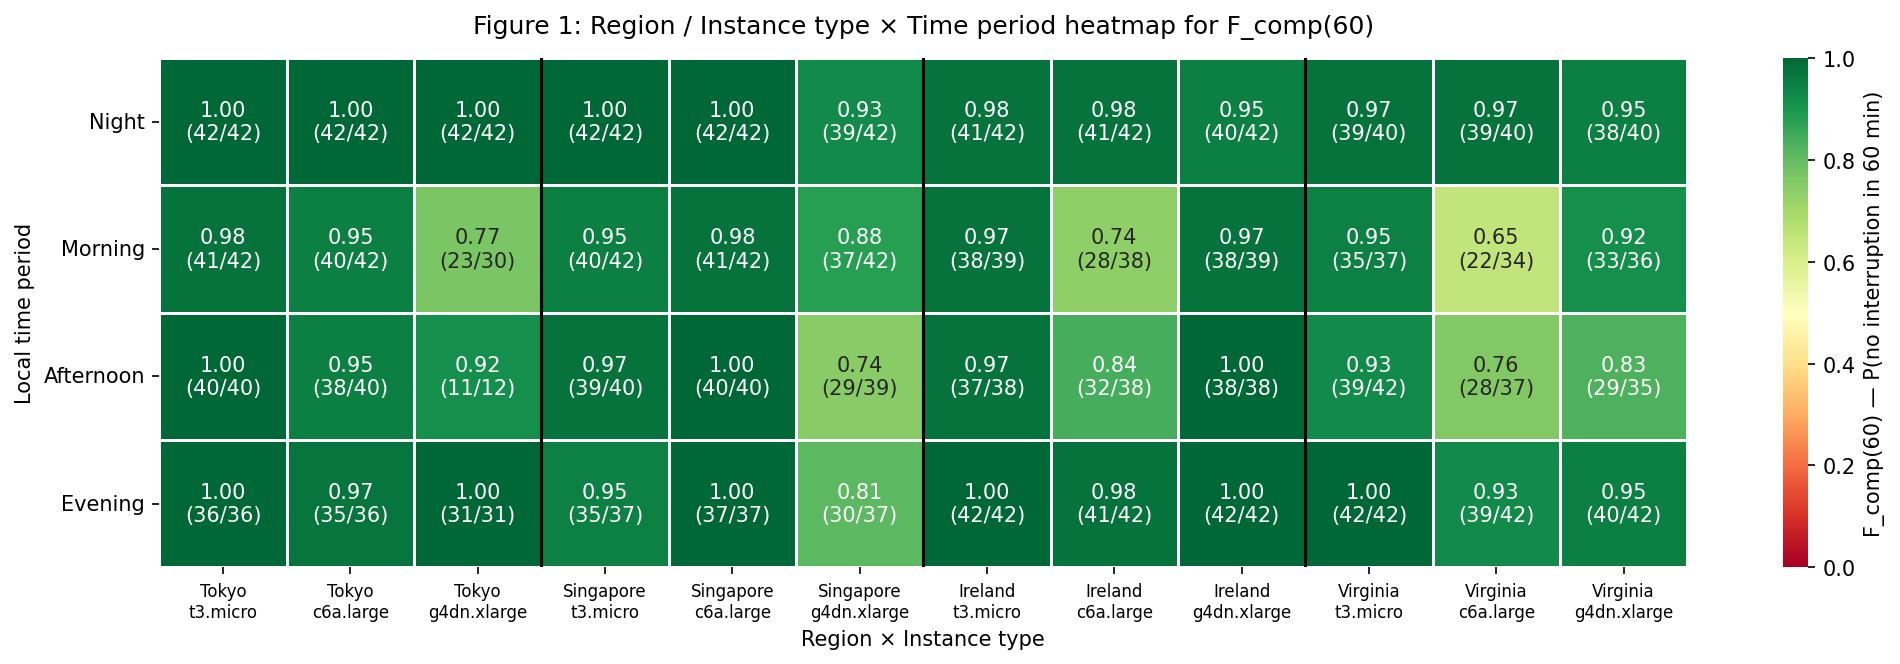
\includegraphics[width=\textwidth]{figure1_fcomp60_heatmap.png}
\caption{$F_{\mathrm{comp}}(60)$ heatmap by local time period, region, and instance type. Annotations show the value and sample counts ($n_{\mathrm{comp}}/n_{\mathrm{succ}}$).}
\label{fig:heatmap_fcomp60}
\end{figure}

\subsection{Time-of-Day Effects on Deadline-Conditioned Completion Feasibility}

Figure~\ref{fig:fcomp_multiregion} shows $F_{\mathrm{comp}}(d)$ for $d \in \{5, 10, 30, 60\}$ minutes for the four region--instance-type combinations with the largest observed time-period variation in $F_{\mathrm{comp}}(60)$.

In panel~(a), N.~Virginia c6a.large, the Night period achieved $F_{\mathrm{comp}}(60) = 0.97$, whereas the Morning period fell to $F_{\mathrm{comp}}(60) = 0.68$, a difference of approximately 0.30. Even at the shortest deadline of $d = 5$ minutes, the Morning period already showed $F_{\mathrm{comp}}(5) = 0.88$, indicating that interruption risk begins to accumulate within the first five minutes. The Night and Evening periods maintained $F_{\mathrm{comp}}(d) \geq 0.93$ across all deadlines.

Panel~(b), Ireland c6a.large, shows a qualitatively similar pattern. The Night period achieved $F_{\mathrm{comp}}(60) = 1.00$ for all deadlines, while the Morning period dropped to $F_{\mathrm{comp}}(60) = 0.76$ and the Afternoon to $0.87$. These results suggest that c6a.large instances in both N.~Virginia and Ireland are more susceptible to interruption during daytime hours.

For g4dn.xlarge in Tokyo (panel~(c)), the Morning period showed the largest degradation with $F_{\mathrm{comp}}(60) = 0.77$, while the Night and Evening periods reached $F_{\mathrm{comp}}(60) = 1.00$. In Singapore (panel~(d)), the Afternoon period exhibited the lowest $F_{\mathrm{comp}}(60) = 0.77$, whereas the Morning was also reduced at $0.88$ compared to Night at $0.95$.

Across all four panels, the Night period consistently achieved the highest or near-highest $F_{\mathrm{comp}}(d)$ values, while the Morning or Afternoon period was associated with the greatest interruption risk depending on the region. These observations provide preliminary evidence that time of day can serve as an operationally meaningful indicator for scheduling short-running workloads on spot instances.

\begin{figure}[t]
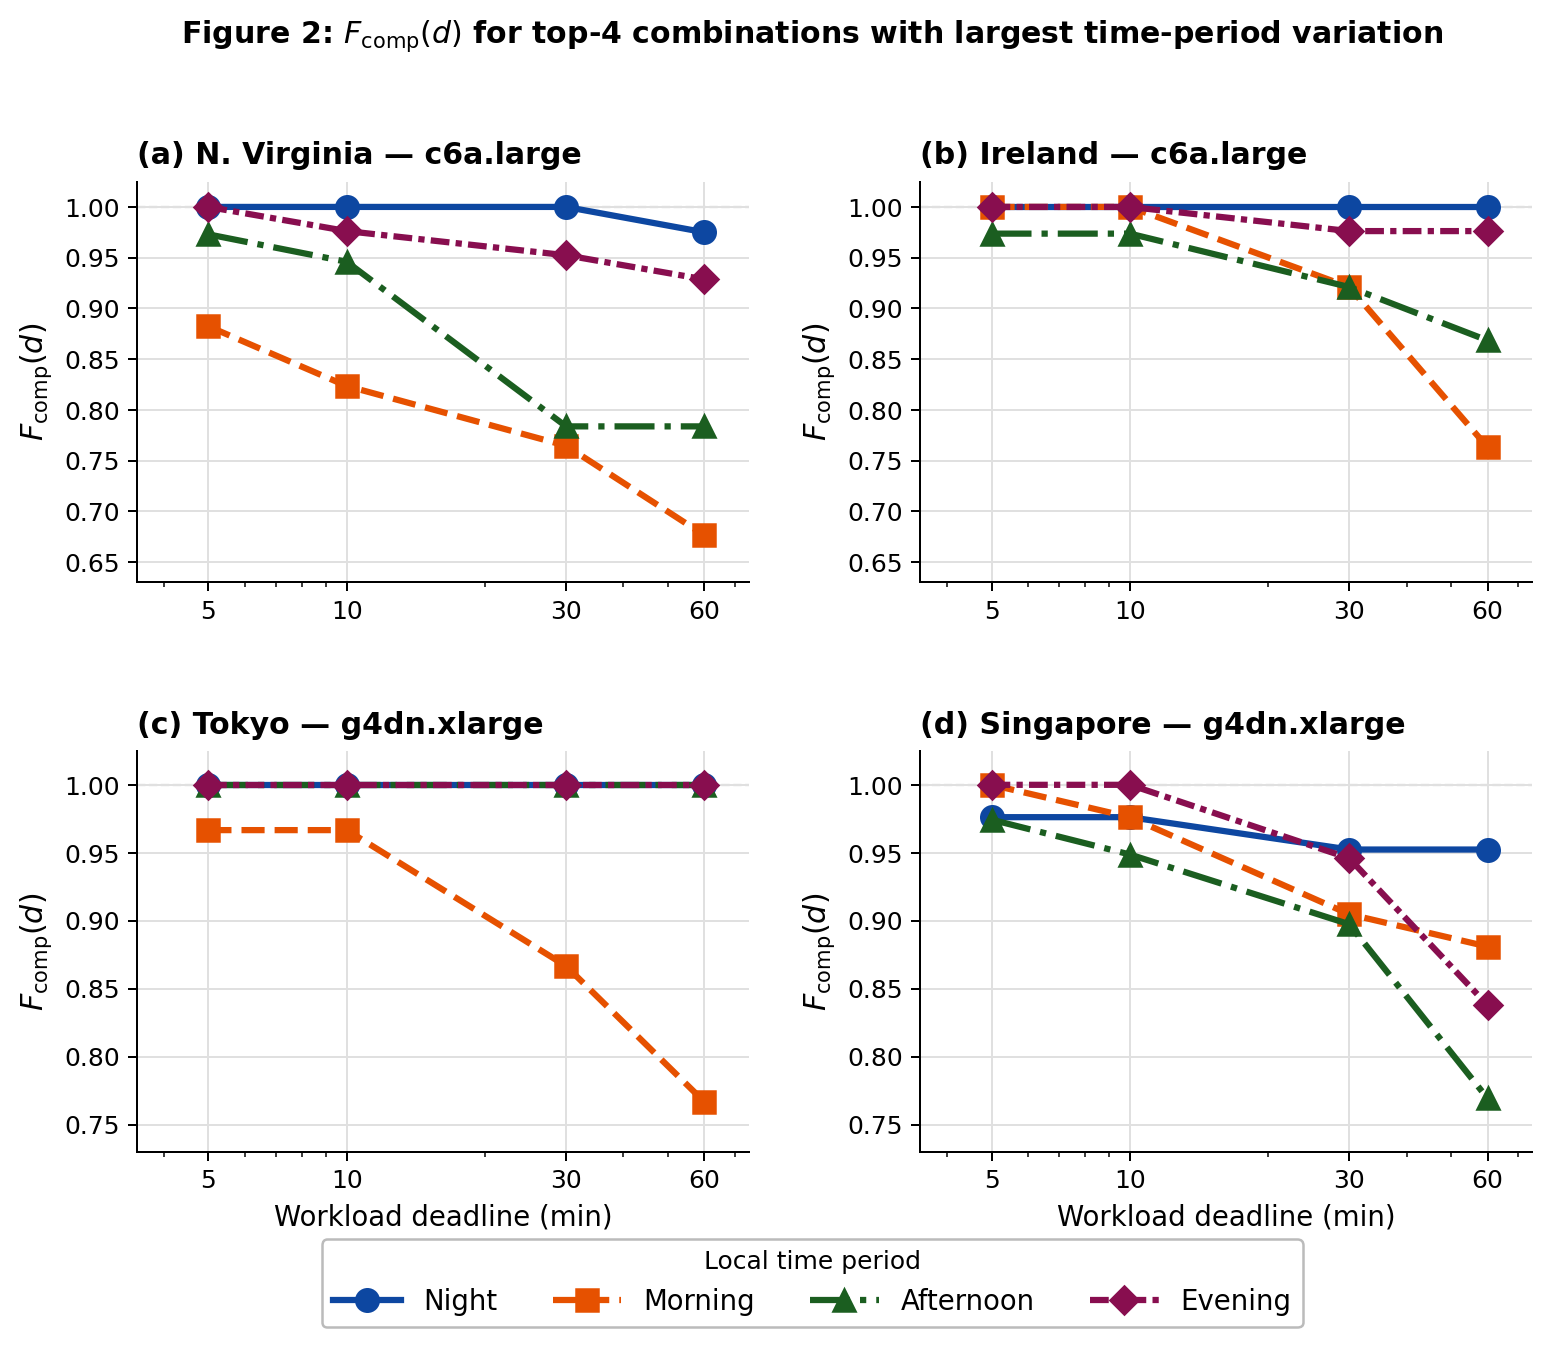
\includegraphics[width=\textwidth]{figure2_fcomp_multiregion.png}
\caption{$F_{\mathrm{comp}}(d)$ for the four region--instance-type combinations with the largest time-period variation. Lines represent local time periods; the x-axis uses a logarithmic scale.}
\label{fig:fcomp_multiregion}
\end{figure}

\section{Discussion}

\subsection{Time-of-Day as an Operational Scheduling Factor}

The results show that $F_{\mathrm{comp}}(d)$ varies substantially by local time period for compute-oriented and GPU-based instance types, while remaining largely stable for t3.micro. The most pronounced differences were observed in N.~Virginia for c6a.large, where the Night period achieved $F_{\mathrm{comp}}(60) = 0.97$ compared to $0.68$ in the Morning—a gap of approximately 0.30. A similar contrast appeared in Ireland ($1.00$ vs.\ $0.76$) and Tokyo g4dn.xlarge ($1.00$ vs.\ $0.77$). These findings suggest that, for workloads with flexible execution timing, selecting the Night period (00:00–05:59 local time) can substantially reduce the risk of interruption before the workload deadline.

The observed pattern is consistent with the hypothesis that local cloud demand follows a diurnal cycle. During local nighttime hours, business-driven demand for compute and GPU capacity is likely lower, leaving more spare capacity available for spot instances. Conversely, the Morning or Afternoon periods—corresponding to the start of local business hours—appear to be associated with increased spot market competition and higher interruption rates. The regional difference in which period is riskiest further supports this interpretation: N.~Virginia and Ireland show Morning as the riskiest period, which aligns with the start of the North American and European business day; Singapore shows Afternoon as riskiest, consistent with peak activity during Asian afternoon hours.

\subsection{Instance Type and Interruption Susceptibility}

The observed robustness of t3.micro ($F_{\mathrm{comp}}(60) \geq 0.95$ in all conditions) contrasts with the higher interruption susceptibility of c6a.large and g4dn.xlarge. This difference may be attributed to the relative demand for each instance type in the spot market. Burstable lightweight instances such as t3.micro are likely to face less competition for spare capacity, whereas compute-optimized and GPU-accelerated instances are in higher demand for machine learning and batch workloads. This is consistent with the findings of Lee et al.~\cite{Lee2022SpotLake}, who reported that GPU instances and large instance types tend to have lower spot availability. Our results extend this finding to the deadline-conditioned perspective: not only are GPU and compute instances more likely to be interrupted, but their interruption risk varies more strongly with time of day than that of lightweight instances.

\subsection{Implications for Workload Scheduling}

These preliminary observations have direct implications for practitioners who use spot instances for short-running workloads with flexible scheduling. For c6a.large or g4dn.xlarge instances in regions such as N.~Virginia, Ireland, or Tokyo, scheduling CI/CD jobs or batch-processing tasks during the Night period can increase $F_{\mathrm{comp}}(60)$ by up to 0.30 compared to the Morning period, without requiring any changes to the workload itself or any provider-specific API calls. Since $F_{\mathrm{comp}}(d)$ is derived solely from directly observed launch and interruption records, this approach provides a transparent and interpretable scheduling signal that complements opaque provider indicators such as SPS.

It should be noted that the riskiest time period differs by region: Morning in N.~Virginia, Ireland, and Tokyo, but Afternoon in Singapore. Users should therefore derive $F_{\mathrm{comp}}(d)$ from their own observed data in the target region rather than applying a single universal rule.

\subsection{Limitations}

Several limitations must be acknowledged. First, the observation period is limited to one week, and the sample size per time period is approximately 30–42 instances per region--instance-type combination. The results may therefore reflect short-term fluctuations in spot capacity and should not be generalized as long-term or seasonal trends. Second, this study uses uninterrupted instance availability as a proxy for workload completion feasibility and does not execute actual application-level workloads. Application-specific factors such as checkpointing, startup overhead, and inter-job dependencies are outside the scope of this study. Third, only one instance was launched per hour for each combination, so concurrent-launch effects and queue behavior under high demand are not captured. Fourth, no maximum spot price was specified, so the results reflect behavior under the default AWS pricing configuration only. Future work should address these limitations by extending the observation period, increasing the sampling frequency, running actual CI/CD workloads, and comparing $F_{\mathrm{comp}}(d)$ against SPS and other provider-specific indicators.

\section{Conclusion}

This paper presented a time-of-day-aware empirical measurement framework for evaluating the completion feasibility of short-running workloads on AWS Spot Instances. Unlike approaches that focus only on launch-time availability or infrastructure-level survival time, this study reformulated spot instance reliability as deadline-conditioned completion feasibility for workload deadlines of 5, 10, 30, and 60 minutes. The proposed framework separately records launch success and runtime interruption behavior across multiple regions and instance types.

The main idea of this study is to treat time of day as an operational variable for deciding when to execute short-running workloads on spot instances. By analyzing launch success rate, interruption-before-deadline rate, deadline-conditioned completion feasibility, and observed availability duration by local time of day, region, and instance type, the proposed approach supports a more interpretable spot instance usage strategy based on directly observed completion behavior. Future work will extend the measurement period, increase the sample size, evaluate actual CI/CD and batch-processing workloads, and compare the observed completion feasibility with provider-specific indicators such as SPS.

% 日本語要約：
% 本稿では，AWS Spot Instances 上における短時間ワークロードの完了可能性を評価するための，時間帯を考慮した実測フレームワークを提案した．
% 本研究では，スポットインスタンスの信頼性を，起動可能性やインフラレベルの生存時間だけでなく，5分，10分，30分，60分の deadline-conditioned completion feasibility として再定義した．
% また，時間帯を短時間ワークロードの実行タイミングを決めるための運用上の変数として扱う点を強調した．
% 今後は，観測期間の延長，サンプル数の増加，実際の CI/CD・バッチ処理ワークロードの評価，SPS との比較を行う予定である．

%
% ---- Bibliography ----
%
\begin{thebibliography}{8}

\bibitem{Lin2022Survey}
Lin, L., Pan, L., Liu, S.:
Methods for improving the availability of spot instances: A survey.
Computers in Industry, 141, 103718 (2022).
\doi{10.1016/j.compind.2022.103718}

\bibitem{Ramesh2025}
Ramesh, D.G.A., Lennon, R.G.:
Evaluating the Impact of Reserved Instances vs. Spot Instances in DevOps Cloud Workflows.
In: 2025 35th Irish Signals and Systems Conference (ISSC).
IEEE (2025).
\doi{10.1109/ISSC67739.2025.112915051}

\bibitem{Garg2025}
Garg, D., Kaata, S.K., Bhumireddy, D.R., Bolla, B.K.:
Reducing Cloud Cost Through Optimized Bidding for AWS Spot Instances.
In: 2025 3rd International Conference on Advances in Computation, Communication and Information Technology (ICAICCIT).
IEEE (2025). \doi{10.1109/ICAICCIT68829.2025.11433986}

\bibitem{Katayama2022}
Katayama, D., Kasai, K., Koita, T.:
Migration Destination Selection Algorithm for Spot Instances using SPS.
In: 2022 IEEE International Conference on Big Data (Big Data),
pp. 6690--6692. IEEE, Osaka (2022).
\doi{10.1109/BigData55660.2022.10020520}

\bibitem{Kim2024SpotInterruption}
Kim, K., Lee, K.:
Making Cloud Spot Instance Interruption Events Visible.
In: Proceedings of the ACM Web Conference 2024 (WWW '24),
pp. 2998--3009. ACM, New York (2024).
\doi{10.1145/3589334.3645548}

\bibitem{Lee2022SpotLake}
Lee, S., Hwang, J., Lee, K.:
SpotLake: Diverse Spot Instance Dataset Archive Service.
In: 2022 IEEE International Symposium on Workload Characterization (IISWC),
pp. 242--255. IEEE (2022).
\doi{10.1109/IISWC55918.2022.00029}

\bibitem{Pham2018}
Pham, T.-P., Ristov, S., Fahringer, T.:
Performance and Behavior Characterization of Amazon EC2 Spot Instances.
In: 2018 IEEE 11th International Conference on Cloud Computing (CLOUD).
IEEE (2018). \doi{10.1109/CLOUD.2018.00017}

\end{thebibliography}
\end{document}
